\section{Analysis of Results}

After completion of the processing portion of this work, the results
must be processed in a useful way, which includes both the biological
implications of the gene calls as well as the computational, or gene
finding features, of the the selected programs. To better understand
how gene finders perform in these two classes, we must define an
appropriate plan for analysis of the results produced so
far. Currently, downstream analysis plan has been broken down into
several sections.

\subsection{Basic Analysis}

Basic analysis of gene finding results is an important part of this
research. Total gene, transcript and protein counts will be identified
for each genome and gene finding tool combination. Comparing the
general outputs of these programs will provide an idea of their
performance in different \textit{Trichoderma} genomes In addition to
these basic outputs, analysis will also be performed for the
following: distribution of gene lengths, intersection of gene calls,
smallRNAs and repetetive regions, shared gene content with a close
fungal relative. Analysis for these results can be performed through
simple shell scripting with grep and other unix tools, although
processing through Python might provide results that are easier to
reproduce with proper programming. Having one script with several
modules that can be rerun at will would be easier to handle than
multiple shell scripts. This thinking for processing will be applied
to subsequent sections of this as well.

\subsection{Distribution of Gene Lengths}

One important aspect of gene finding tools to consider is the
distribution of gene lengths predicted by each individual
tool. Certain tools, such as GeneMark are based on pre-defined models,
which may limit the length of predicted genes, while tools such as
Braker2, which incorporate RNAseq data, may predict a wider
distribution of gene lengths depending on the input dataset
used. Regardless, the ability of a gene finding tool to predict a
wider range of gene lengths can be usefull if users are looking for
short or larger genes. To help determine whether or not these tools
find shorter genes, or small RNAs, the genomes of interest have been
annotated using Infernal along with the Rfam database to identify
small RNAs as a ground truth. These annotation results will also be
included with results from other annotation processes further down the
line. Again, these results can be produced with a Python script. The
resulting data could then be used as input to violin plots for each
genome and set of tools considered in this analysis process. Violin
plots should provide a good visualization of gene lengths as well as
the number of genes found with specific lengths. Means could also be
compared staatistically for genomes and the mutliple tools considered
as well.

Analysis of gene lengths was performed using a Python script. Combined
predicted CDS sequences for each predicted gene were used as input for
the total gene length. CDS sequences predicted by Braker2, were
directly available in the output directories when the program was
run. CDS sequences from GeneMark required extraction of the CDS
sequences from the genome FASTA files. This process was performed
using the gffread tool from the Cufflinks package. Predicted CDS
sequences were loaded into Python using Biopython's SeqIO
package. Sequence lengths were then placed in a list and analyzed
using a combination of pandas and numpy. A log10 transformation was
applied to the sequence lengths as the original distribution was
heavily skewed due to long outlier CDS sequences. After
transformation, the CDS length distribution appears as a normal
distribution, although there are interesting troughs that occur in
several of the peaks for several of the genomes considered. These
troughs did not appear in a comparable Yeast reference dataset,
although the log transformed data still appears to be a normal
distribution.

\subsection{Intersection of Gene Calls, smallRNAs and Repetitive Regions}

Annotation of all three features in the title are important in
assessing the ability of gene finding tools. Even more important, is
the potential for for overlap between gene calls and small RNAS as
well as repetitive regions the genomes. As discussed in the previous
subsection, the distribution of gene lengths predicted by a gene
finding tool can be an important metric for users. Overlapping
predicted genes from tools alongside the output from Infernal and the
Rfam database may provide insight into whether or not these gene
finding tools are able to predict RNAs of very short length. In
addition to small RNAs, repetitive regions in \textit{Trichoderma}
genomes hold potential for recombination and gene content, although
the inherent nature of these repetitive regions (low nucleotide
diveristy) suggests that gene content should be low, based on the
nucleotides required for start and stop codons. Analysis of these
intersections can be perfomed via bedtools or through biopython (I
believe). Again, having all processing steps included in one script as
separate functions that can be called at whim will make further
processing easier if changes need to be made.

\subsection{Methodology for Indetifying Overlapping Features}

To analyze the results from multiple gene-finding tools, we must first
define two conceptual topics.

Definition of a Feature: First, a feature, in the context of this
research, is any item contained within a Genomic Feature Formated file
(GFF). Each feature contains a contig ID, a start position, end
position, and a feature ID based on the information from the GFF
file. These features will be used in the process of identifying
regions, or overlapping features from prediction tools.

Definition of a Region: Secondly, a region is defined as any overlap
between features relative to the reference sequence being
considered. To identify regions, every feature from each GFF file
being considered, is sorted by start position. For clarification, the
start position is based on the left most position in the GFF file,
regardless of the strand that the feature is predicted on. Once the
features have been sorted by left position, the sorted features are
iterated over to identify regions, as long as the left position of the
next feature is consistent with the left position , within the left
and right position, or equal to the right position of the current
region. One drawback to this approach is that ideally, identification
of overlap types based on Allen's interval algebra would be performed
at this point. However, the methodology of initially sorting features
based on left position somewhat prevents this process from
happening. This implementation requires further processing of
identified regions late on the process, simplifying the all to all
comparison that would occur if all features were considered at once.

Identification of overlapping features results in different 'classes'
of regions. A few basic cases are outlined in figure
~\ref{fig:igv-cases}. The simplest of case is the a region where the
gene finders agree unanimously on the gene (agreement currently means
same start and end point). 


\begin{figure}[b]
  \centering
  \begin{subfigure}{0.9\textwidth}
    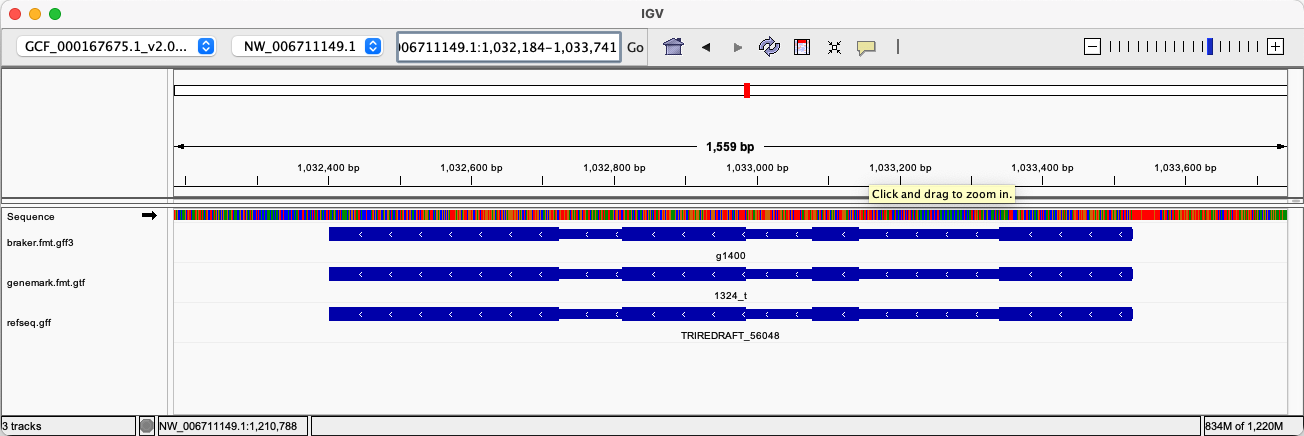
\includegraphics[width=\textwidth]{figures/igv/igv-agreement-thin.png}
    \label{fig:igv-agree}
    \caption{Complete Agreement}
  \end{subfigure}
  \begin{subfigure}{0.9\textwidth}
    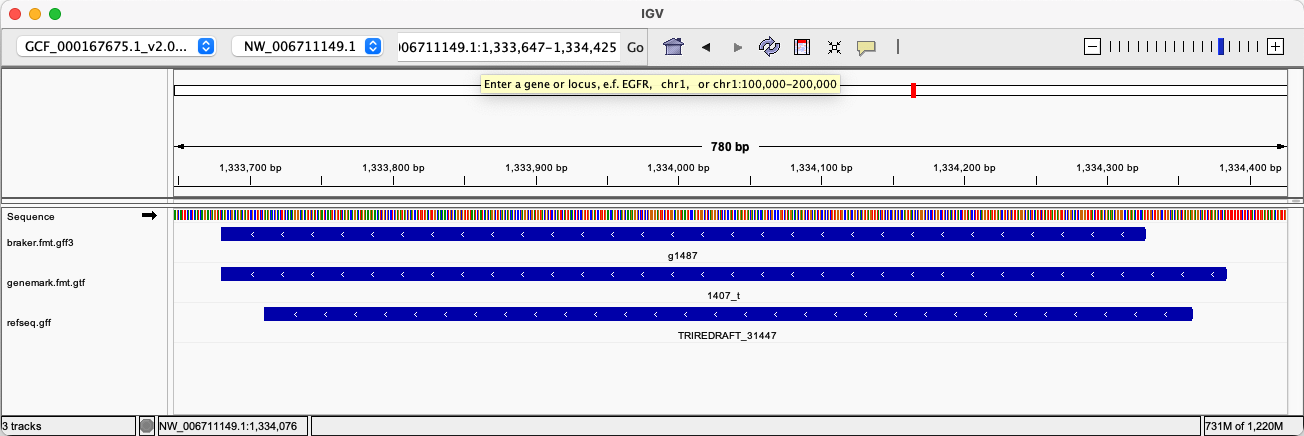
\includegraphics[width=\textwidth]{figures/igv/igv-start-stop-thin.png}
    \label{fig:igv-start-stop}
    \caption{Start/Stop Disagreement}
  \end{subfigure}
  \phantomcaption
\end{figure}
\begin{figure}[t]
  \ContinuedFloat
  \centering
  \begin{subfigure}{0.9\textwidth}
    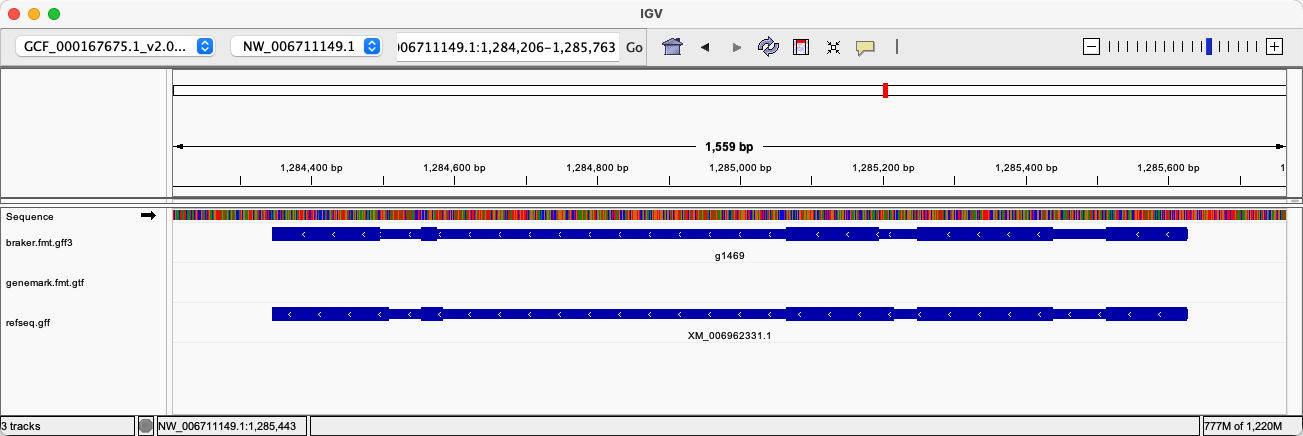
\includegraphics[width=\textwidth]{figures/igv/igv-missing-thin.png}
    \label{fig:igv-missing}
    \caption{Missing Prediction}
  \end{subfigure}
  \begin{subfigure}{0.9\textwidth}
    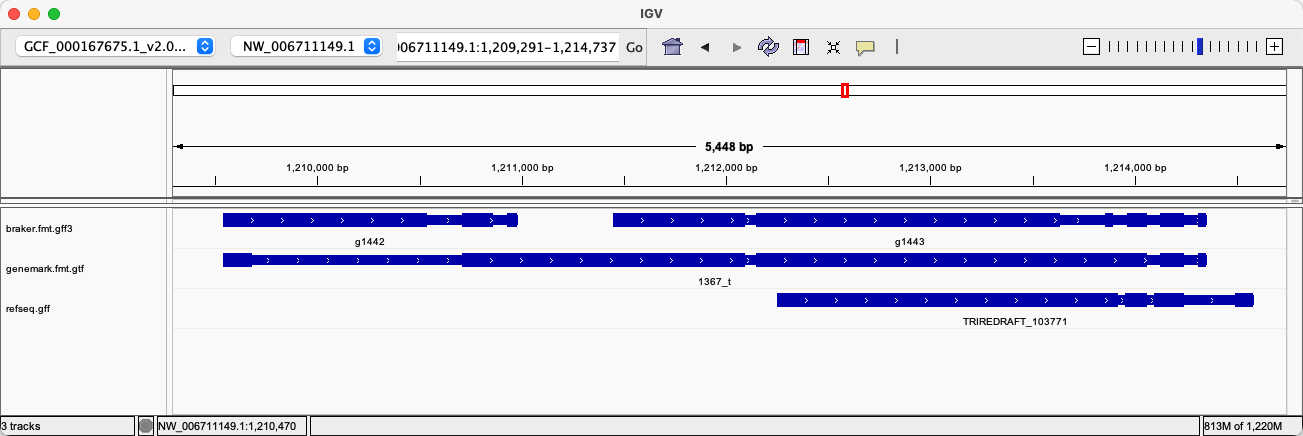
\includegraphics[width=\textwidth]{figures/igv/igv-complicated-thin.png}
    \label{fig:igv-complicated}
    \caption{Complete Disagreement}
  \end{subfigure}
  \caption[Examples of Potential Regions]{Several visual examples of
    regions using IGV. \textbf{a)} Region where all prediction tools
    are in agreement. \textbf{b)} Prediction tools agree that gene is
    present, but not on the exact start and/or stop
    positions. \textbf{c)} A region where one tool does not predict a
    gene while the others do. \textbf{d)} A region with a combination
    of disagreeing predictions.}
  \label{fig:igv-cases}
\end{figure}

\subsection{Shared Gene Content with Closely Related Organisms}

While considering novel gene calls can be useful, comparing those
calls to a well-studied close relative can provide a rudimentary
validation of the calls as a ground truth. This process will confirm
that at least most of a closely related fungal genome's coding
sequences are predicted and shared by the gene calls for
\textit{Trichoderma}. Results for this processing can be produced with
a simple BLAST search and apropriate cutoff values (i.e. query
coverage, percent identity, E-score, etc.). While running BLAST is a
simple process, the selection of a closely related organism is more
difficult. One initial choice would be to work with
\textit{Saccharomyces cerevisiae}, or bakers yeast, as it is extremely
well studied and would be considered a model organism, similar to
\textit{Arabidopsis} and \textit{Mus musculus}. However,
\textit{Saccharomyces cerevisiae} diverged evolutionarily millions of
years ago, which may make it a poor candidate for a comparative
analysis. The second candidate considered for comparison is
\textit{Fusarium avenaceum}, as it is also well studied an more
closely related to \textit{Trichoderma} than yeast, and has a genome
similar in size to that of \textit{Trichoderma} species, at roughly
40Mb. Finally, comparison of assemblies and predicted genes to another
\textit{Trichoderma} strain is a reasonable approach. In this case,
\textit{Trichoerma atroviride} was selected as it is not included in
the species used in the gene prediction portion of this analysis. From
these assemblies, the RefSeq proteins (queries) from NCBI will be used
in a tblastn search against each genome sequence from DC1, Tsth20,
\textit{T.reesei}, \textit{T. harzianum}, and \textit{T. virens}
(subjects). Resulting BLAST hits will then be filtered based on
suitable alignment coverage and identity, which will be determined by
the reference sequence being considered. Total number of BLAST hits
reported for each organism will provde information about completeness
of assemblies and overall coverage of the gene/coding sequence space
in the query sequences (need to be clear with language used for blast
subjects and query). In addition, BLAST hits will be analysed with the
region identification approach to identify coverage of protein and coding
sequences in relation to gene predictions generated previously.

\subsection{BUSCO Analysis}
Another method for assessing the completeness of a set of predicted
genes is Benchmarking Universal Single-Copy Orthologue (BUSCO)
analysis\cite{10.1093/molbev/msab199}. BUSCO analysis is similar to
analysis of overlapping or shared gene content with a close relative
in that we are comparing the predicted gene sets to an existing
standard or reference. With BUSCO analysis, the reference set has a
far more strict definition. The datasets used for BUSCO analysis are
based on single-copy orthologs generally found in an genome of
interest. What this means is that BUSCO searches for single-copy genes
that should be present in an organism based on the database selected
for analysis. As an example in fungi, if one were interested in
assessing the completeness of their annotated genes in a similarly
related fungi, there should be a set, or subset, of single-copy genes
present in the new annotation that are expected to be present after
evolutionary divergence(...). This can be thought of as similar to a
'core' gene set. Results from BUSCO analysis are typically reported in
a percentage of the gene set included in the BUSCO
dataset. Percentages of single and duplicated hits are reported as
well. While a high reported coverage of the BUSCO dataset is
considered good, it is not fully indicative of excellent gene finding
performance

\subsection{Comparative Genomics}

With the data produced by this research, it is possible to perform som
commparative genomics (time permitted), mostly related to the
assemblies generated during this work along with the RefSeq genomes
included from NCBI. Mummer is a potential tool to use for all to all
genome alignments, although there may be difficulty in the ordering of
contigs/scaffolds/chromosomes when performing thes alignments. This
work is not necessarily required but would be interesting from a
biological perspective to identify rearrangements, inversions and
such.
